\documentclass[12pt]{article}

\usepackage[a4paper,margin=2cm,top=2cm,bottom=2cm,xetex]{geometry}
\usepackage[utf8]{inputenc}
\usepackage{color,xcolor}
\usepackage{enumitem}
\usepackage{amssymb}
\usepackage{amsthm}
\usepackage{amsfonts}
\usepackage{mathtools}
\usepackage{flexisym}
\usepackage{algorithm}
\usepackage{pdfpages}
\usepackage{algorithmic}
\usepackage{tabularx}
\usepackage{xepersian}
\usepackage{amsmath}
\usepackage{physics}
%\usepackage{mathtools}

\DeclareFontFamily{U}{matha}{\hyphenchar\font45}
\DeclareFontShape{U}{matha}{m}{n}{ <-6> matha5 <6-7> matha6 <7-8>
matha7 <8-9> matha8 <9-10> matha9 <10-12> matha10 <12-> matha12 }{}
%\DeclareSymbolFont{matha}{U}{matha}{m}{n}
%
%\DeclareMathSymbol{\nvartrianglelefteq}{\mathrel}{matha}{"9E}
%\DeclareMathSymbol{\vartrianglelefteq}{\mathrel}{matha}{"9C}

\newcount\HWcnt
\def\ttmp#1#2#3#4#5#6#7#8#9|{\def\Wjob{#9}}%
\expandafter\ttmp\jobname |
\def\ttmp#1#2#3{\global\HWcnt=#2#3}
\expandafter\ttmp\Wjob

\settextfont[Scale = 1.0 ,
             BoldFont = *Bd ,
             ItalicFont = *It ,
             BoldItalicFont = *BdIt ,
             Extension = .ttf
            ]{XB Niloofar}
\ExplSyntaxOn
\cs_set_eq:NN
\etex_iffontchar:D
\tex_iffontchar:D
\cs_undefine:N \c_one
\int_const:Nn \c_one { 1 }
\ExplSyntaxOff
\setdigitfont[Scale = 1.0 ,
             BoldFont = *Bd ,
             ItalicFont = *It ,
             BoldItalicFont = *BdIt ,
             Extension = .ttf
            ]{XB Niloofar}
\renewcommand{\baselinestretch}{1.2}
\pagestyle{empty}

\makeatletter
\def\abj@num@i#1{%
    \ifcase #1\or الف\or ب\or ج\or د\or ه\or و\or ز\or ح\or ط\fi \ifnum #1=\z@ \abjad@zero \fi
}
\renewcommand{\theenumi}{\abjad{enumi}}
\renewcommand{\labelenumi}{\theenumi)}
\long\def\makeHead#1{%
	\begin{center}\large
		\begin{tabular}{@{}p{.33\linewidth}<{\hfill}@{}>{\hfil}p{.33\textwidth}<{}@{}>{\hfill}p{.33\textwidth}@{}}
            \textbf{محاسبات عددی} & & \textbf{سری شمارهٔ 3} \\[.5ex]
            \textbf{نیم‌سال دوم ۱۴۰۱-۱۴۰۲} & &  \textbf{موعد تحویل: #1}\\[.5ex] \hline\hline
		\end{tabular}
	\end{center}\smallskip
%	\def\theenumii{\arabic{enumii}}\def\theenumi{\alph{enumii}}\def\labelenumi{\theenumi)}\def\labelenumii{\theenumii)}%
}

\newcommand{\Rule}{\ \hfill\rule{\linewidth}{0.5pt}\hfill\ \par\vspace*{-2ex}\par}
\newcommand{\DescRule}{\ \hfill\rule{\linewidth}{1pt}\hfill\ \vspace*{-2ex}\par}
\def\rank{\mathop{\mathrm{rank}}\nolimits}

\begin{document}
\makeHead{پاسخنامه تمرین}
\begin{description}
% 	\item{\textbf{سوال 1.}} \input{\jobname-q1.tex}
	
% 	\Rule
	\item{\textbf{سوال ۱.}}
	گزاره‌های زیر را اثبات کنید:
\begin{enumerate}
	\item
	در صورتی که 
	$f[x_0,x_1,x_2,...,x_n]$
	تفاضلات تابع دلخواه 
	$f$
	در نقاط 
	$x_0$
	تا
	$x_n$
	باشد،
	
	
	$f[x_0,x_1,...,x_n] = \sum_{i=0}^{n}\frac{f(x_i)}{ \displaystyle  \prod_{j=0 \atop j\neq i}^{n}(x_i - x_j)}$
	
	\item
	فرض کنید 
	$f$
	در بازه‌ی شامل 
	$x_0,x_1,...x_n$،
	$n$
	بار مشتق‌پذیر است. در این صورت به ازای 
	$\xi$
	در بازه‌ی شامل نقاط
	$x_0,x_1,...,x_n$
	ثابت کنید:
	
	\begin{center}
		$f[x_0,...,x_n] = \frac{f^{(n)}(\xi)}{n!}$
	\end{center}
\end{enumerate}

\textcolor{blue}{حل
\begin{enumerate}
    \item 
    می‌دانیم در روش
    \LR{Divided Difference}:
    \begin{align} \label{eq:1}
        \text{چندجمله‌ای درونیابی} = f(x_0) + (x - x_0) f[x_0, x_1] + \dots + (x - x_0) \dots (x - x_n) f[x_0, \dots, x_n]
    \end{align}
    پس عبارت فوق چندجمله‌ای از درجه
    $n$
    است که ضریب 
    $x^n$
    در آن برابر 
    $f[x_0, \dots, x_n]$
    است. 
    \\
    اما اگر سوال را با لاگرانژ حل می‌کردیم:
    \begin{align*}
    \text{درونیابی شده
    $f$} = \sum_{i = 0}^{n} L_i (x) f(x_i) = 2 \stackrel{L_i(x) = \prod_{j = 0 \neq i}^{n} \frac{(x - x_j)}{(x_i - x_j)}}{=} \sum_{i = 0}^{n} (\prod_{j = 0 \neq i}^{n} \frac{(x- x_j)}{(x_i - x_j)}) f(x_i)
    \end{align*}
    با توجه به این که پشت
    $x$
    ها عددی نیست، ضریب 
    $x^n$
    برابر جمع ضرایبی است که به کل کسر اعمال می‌شود یعنی
    $\sum_{i = 0}^{n} \prod_{j = 0 \neq i}^{n} \frac{1}{(x_i - x_j)} f(x_i)$.
    به عبارت دیگر در عبارت درون‌یابی شده، پشت 
    $x^n$
    عدد فوق واقع است. از طرفی می‌دانیم
    جواب
    \LR{interpolation}
    در این دو روش یکسان (یونیک) است، پس ضریب 
    $x^n$
    در
    \LR{Divided Difference}
    که برابر با
    $f[x_0, \dots, x_n]$
    است، با ضریب 
    $x^n$
    در روش لاگرانژ باید برابر باشد وگرنه چندجمله‌ای یکی نخواهد بود. در نهایت داریم
    \begin{align*}
        f[x_0, \dots, x_n] = \sum_{i = 0}^{n} \prod_{j = 0 \neq i}^{n} \frac{1}{(x_i - x_j)} f(x_i) = \sum_{i = 0}^{n} \frac{f(x_i)}{\prod_{j = 0 \neq i}^{n} (x_i - x_j)}
    \end{align*}
    \item 
    از رابطه
    \ref{eq:1}
    بخش قبل اقدام می‌کنیم
    (روش 
    \LR{Divided Difference}).
    تابع 
    اینترپولیشن روی نقاط
    $x_0$
    تا
    $x_n$
    است، پس در این نقاط تابع
    $f$
    اصلی با اینترپولیشن خود (تعریف کنیم برابر با
    $P_n(x)$)
    برابر است. پس تابع
    $P_n(x) - f(x)$,
    $n + 1$
    ریشه دارد. می‌دانیم بین هر دو ریشه چنین تابعی که مشتق‌پذیر و پیوسته است، مشتق صفر است.
    پس اگر در 
    $n + 1$
    نقطه ریشه داشته باشد، بین هر دوتا در یکی مشتق صفر است پس در کل در 
    $n$
    نقطه مشتق صفر است. مشابها از روی همین 
    $(P_n(x) - f(x))^{'}$
    اگر مشتق بگیریم، در 
    $n - 1$
    نقطه مشتق آن صفر است، و به همین شکل مشتق 
    $n$
    ام 
    $P_n(x) - f(x)$
    در یک نقطه که آن را همان
    $\xi$
    فرض می‌کنیم صفر است (مشخصا 
    $\xi$
    در بین این نقاط است زیرا در هر مرحله جایی که مشتق صفر می‌شد بین همان نقاط قبلی بود). در این نقطه‌ی 
    $\xi$،
    مقدار مشتق 
    $n$
    ام 
    $f$
    و
    $P_n$
    برابر است. یعنی
    \begin{align*}
        f^{(n)}(\xi) =\overbrace{n(n-1) \dots (1)}^{n!} f[x_0, \dots,x_n] \xRightarrow{(n! \neq 0)} f[x_0, \dots ,x_n] = \frac{f^{(n)}(\xi)}{n!}
    \end{align*}
    در حل این سوال از تمرین‌های قرار داده شده در سایت درس از سال‌های قبل آموخته شده است.
\end{enumerate}
}


	
	\Rule 
	
	\item {\textbf{سوال ۲.}}
	\\
جدول مقادیر زیر را در نظر بگیرید:

\begin{latin}
\begin{table}[H]
  \begin{center}
    \begin{tabular}{c|c c c}
      \textbf{$x$} & $0$ & $1$ & $2$ \\
      \hline
      \textbf{$f(x)$} & 9.90 & 7.94 & 23.00 \\
    \end{tabular}
  \end{center}
\end{table}
\end{latin}

\begin{enumerate}
	\item
	به‌کمک سری تیلور تقریبی از
    $f''(1)$
    ارائه دهید.
	
	\item
	حد بالای خطای این تقریب را به‌کمک خطای سری تیلور به دست آورید.
\end{enumerate}
\textcolor{blue}{حل
\\
\begin{enumerate}
    \item
    عملا فرمولی که با سری تیلور به آن می‌رسیم همان فرمول نقطه میانی‌ای است که به شکل زیر است:
    \begin{align*}
        f^{''}(x_i) &= \frac{f(x_{i + 1}) - 2f(x_i) + f(x_{i - 1})}{h^2} \\
        &= \frac{23 - 2 (7.94) + 9.9}{1^2} = 17.02
    \end{align*}
    \item
    \begin{align*}
        f(x_i + h) + f(x_i - h) &= \text{جملات توان زوج 
        $h$} \\
        &= 2f(x_i) + h^2 f^{''}(x_i) + \frac{h^4}{4!} \times 2 f^{(4)}(\zeta) \xrightarrow{h = 1}  \frac{1}{12} f^{(4)}(\zeta)
    \end{align*}
    کران بالای بدست آمده به ازای 
    $\zeta$
    در بازه 
    $[x_i, x_i + h]$
    برقرار است.
\end{enumerate}
}
	
	\Rule
	
	\item {\textbf{سوال ۳.}}
	\\
معادله‌ی خطی
$Ax = b$
را با مقادیر زیر درنظر بگیرید:
\begin{LTR}
\begin{center}
A = $\begin{pmatrix}
4 & 1 & -2\\
-1 & 4 & -1\\
1 & -1 & 4
\end{pmatrix}$ و
b =  $\begin{pmatrix}
4\\
0\\
4
\end{pmatrix}$
\end{center}
\end{LTR}

\begin{enumerate}
\item
با تقریب اولیه‌ی
$x^{(0)} = 0$
و سه تکرار از روش ژاکوبی
\footnote{Jacobi}
مقادیر
$x^{(1)}$
،
$x^{(2)}$
و
$x^{(3)}$
را محاسبه کنید.

\item
با تقریب اولیه‌ی
$x^{(0)} = 0$
و سه تکرار از روش گاوس-سایدل
\footnote{\lr{Gauss-Seidel}}
مقادیر
$x^{(1)}$
،
$x^{(2)}$
و
$x^{(3)}$
را محاسبه کنید.
\item
کدام یک از روش‌های بالا تقریب بهتری از جواب‌ها می‌دهد؟

\end{enumerate}

\textcolor{blue}{حل
\\
\begin{enumerate}
    \item دور اول:
    \begin{align*}
        \begin{cases}
        4x_1 + 0 - 2 (0) = 4 \\
         -(0) + 4x_2 - (0) = 0 \\
        0 - (0) + 4x_3 = 4
        \end{cases}
        \Rightarrow 
        \begin{cases}
            x_1 = 1 \\
            x_2 = 0 \\
            x_3 = 1
        \end{cases}
    \end{align*}
    دور دوم:
    \begin{align*}
        \begin{cases}
            4x_1 + 0 - 2(1) = 4 \\
            -1 + 4x_2 - 1 = 0 \\
            1 - 0 + 4x_3 = 4
        \end{cases} \Rightarrow 
        \begin{cases}
            x_1 = 1.5 \\
            x_2 = 0.5 \\
            x_3 = 0.75
        \end{cases}
    \end{align*}
    دور سوم:
    \begin{align*}
        \begin{cases}
            4x_1 + 0.5 - 2(0.75) = 4 \\
            -1.5 + 4x_2 - 0.75 = 0 \\
            1.5 - 0.5 + 4x_3 = 4
        \end{cases}
        \Rightarrow \begin{cases}
            x_1 = 1.25 \\
            x_2 = 0.5625 \\
            x_3 = 0.75
        \end{cases}
    \end{align*}
    \item دور اول:
    \begin{align*}
        &4x_1 + 1 (0) - 2 (0) = 4 \rightarrow x_1 = 1 \\
        &-1 (x_1) + 4x_2 - 1(0) = 0 \rightarrow 4x_2 = x_1 \xrightarrow{x_1 = 1} x_2 = 0.25 \\
        &x_1 - 1(x_2) + 4x_3 = 4 \xrightarrow{(x_1, x_2) = (1,0.25)} 1 - 0.25 + 4x_3 = 4 \rightarrow x_3 = 0.8125
    \end{align*}
    دور دوم:
    \begin{align*}
        &4x_1 + 0.25 - 2(0.8125) = 4 \rightarrow x_1 = 1.34375 \\
        &-x_1 + 4x_2 - 0.8125 = 0 \xrightarrow{\text{از بالایی}} x_2 = 0.5390625 \\
        &x_1 - x_2 + 4x_3 = 4 \xrightarrow{\text{از بالایی ها}} x_3 = 0.798828125
    \end{align*}
    \newpage
    دور سوم:
    \begin{align*}
        &4x_1 + 0.5390625 - 2(0.798828125) = 4 \rightarrow x_1 = 1.2646484375 \\
        &-x_1 + 4x_2 - 0.798828125 = 0 \xrightarrow{\text{از بالایی}} x_2 = 0.5158691406 \\
        &x_1 - x_2 + 4x_3 = 4 \xrightarrow{\text{از بالایی ها}} x_3 = 0.8128051758
    \end{align*}
    \item 
    جواب‌ واقعی (بدست امده از ولفرام)
    \begin{align*}
        \begin{cases}
            x_1 = 1.2753623188 \\ 
            x_2 = 0.5217391304 \\
            x_3 = 0.8115942029
        \end{cases}
    \end{align*}
    حال اختلاف‌ جواب‌های روش‌های بخش الف و ب را مقایسه می‌کنیم
    \\
    اختلاف روش گاوس سایدل:
    \begin{align*}
        \begin{cases}
            \Delta x_1^{A} = 0.0107138743 \\
            \Delta x_2^{A} = 0.0058699898 \\
            \Delta x_3^{A} = 0.0012109729
        \end{cases}
    \end{align*}
    اختلاف روش ژاکوبی:
    \begin{align*}
        \begin{cases}
            \Delta x_1^{B} = 0.0253623188 > \Delta x_1^{A} \\
            \Delta x_2^{B} = 0.0407608696 > \Delta x_2^{A} \\
            \Delta x_3^{B} = 0.0615942029 > \Delta x_3^{A}
        \end{cases}
    \end{align*}
    به وضوح جواب‌های بدست آمده از (ب) نزدیکتر هستند، پس گاوس سایدل تقریب بهتری از جواب‌ها می‌دهد.
\end{enumerate}
}
	
	\Rule
	
	\item {\textbf{سوال ۴.}}
	\\
مقادیر
$f$
در نقاط مختلف در جدول زیر آمده است:

\begin{latin}
\begin{table}[H]
  \begin{center}
    \begin{tabular}{c|c c c c c}
      \textbf{$x$} & $1.2$ & $1.3$ & $1.4$ & $1.5$ & $1.6$ \\
      \hline
      \textbf{$f(x)$} & 0.1823216 & 0.2623642 & 0.3364722 & 0.4054651 & 0.4700036 \\
    \end{tabular}
  \end{center}
\end{table}
\end{latin}

\begin{enumerate}
	\item
    مقدار تقریبی
    $\int\limits^{1.6}_{1.2}f(x)dx$
    را به‌روش سیمپسون محاسبه کنید.
    
    \item
    خطای تقریب بالا را به دست آورید.
\end{enumerate}
\textcolor{blue}{حل
\\
\begin{enumerate}
    \item
    \begin{align*}
        \text{جواب} &\approx \frac{h}{3} (y_0 + y_{2m} + 2(y_2 + y_4 + \dots + y_{2m - 2}) + 4(y_1 + y_2 + \dots + y_{2m - 1})) \\
        &= \frac{0.1}{3} (0.1823216 + 0.4700036 + 2 (0.3364722) \\
        &+ 4(0.2623642+0.4054651)) = 0.13321956 
    \end{align*}
    \item 
    طبق اسلاید ۲۵ لکچر انتگرال:
    \begin{align*}
        |\frac{(b-a)h^4}{180} f^{(4)} (\zeta)| = |\frac{(1.6 - 1.2)(0.1)^4}{180} f^{(4)}(\zeta)| = |\frac{0.00004}{180} f^{(4)}(\zeta)|
    \end{align*}
    به ازای
    $1.2 < \zeta < 1.6$
\end{enumerate}
}
	
	\Rule
	
	\item {\textbf{سوال ۵.}}
	\begin{enumerate}
\item \label{second} دستگاه زیر را با روش 
گاوس-سیدل
\footnote{Gauss-Seidel}
حل کنید.
    \begin{center}
        \begin{cases}
          x - 2y = 4\\
          2x + y = 3
        \end{cases}
    \end{center}
\item \label{first} 
دستگاه زیر را با روش 
گاوس-سیدل
حل کنید
\begin{center}
    \begin{cases}
      2x + y = 3 \\
      x - 2y = 4
    \end{cases}
\end{center}
\item 
چرا با آن که دستگاه‌های 
(الف)
و
(ب)
جواب‌های یکسان دارند ولی همگرایی روش تکرار گاوس-سیدل در 
(الف)
و
(ب)
متفاوت است؟
\end{enumerate}
\noindent \hspace{0.5em} * در 
(الف)
و
(ب)
تقریب اولیه را
$x^{(0)} = y^{(0)} = 0$
در نظر بگیرید.

\textcolor{blue}{
حل 
\\
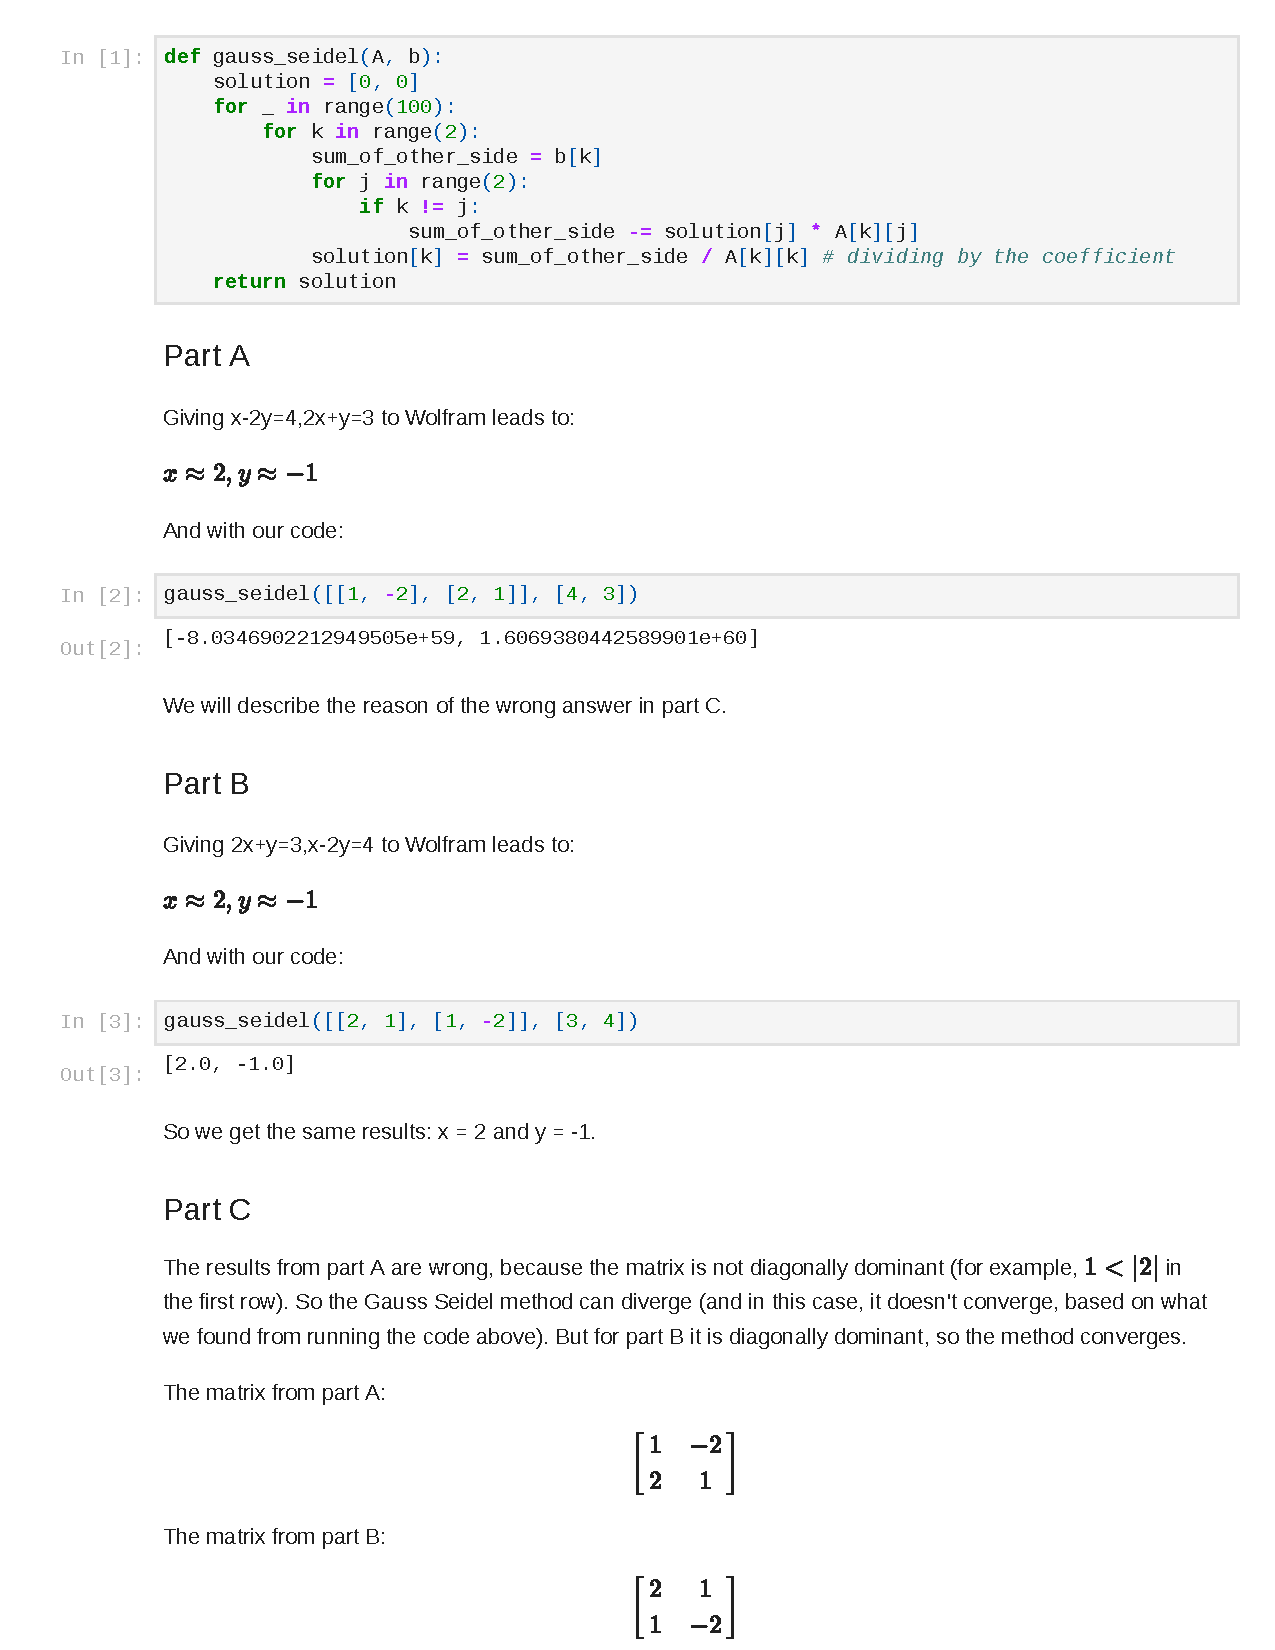
\includepdf[pages={1-},scale=1]{q5.pdf}
}
	
	\Rule

	\vspace*{-2ex}\ \hfill\textbf{موفق باشید.}
\end{description}
\end{document}